\section{Facial Landmark Detection}

Before we can morph one face into another, we need to know \emph{where} the key facial features are located in each image. This is the job of \textbf{facial landmark detection}.

\subsection{What Are Facial Landmarks?}

Facial landmarks are \textbf{semantically meaningful points} on a face. Each landmark marks an anatomically identifiable location, such as:

\begin{itemize}
    \item The corners of the eyes (inner and outer canthus)
    \item The tip and nostrils of the nose
    \item The corners and midpoints of the lips
    \item The outer boundary of the jawline
    \item The arcs of the eyebrows
\end{itemize}

Why do we need them? Because face morphing is fundamentally about establishing \textbf{correspondence}: for every pixel on face~A, we need to know which pixel on face~B plays the same anatomical role. Landmarks give us a sparse set of anchor points that define this correspondence.

\begin{definition}[Corresponding Points]
    Two landmarks $p_i^{(A)}$ and $p_i^{(B)}$ on two different faces are called \textbf{corresponding points} if they refer to the \textbf{same anatomical location}. For example, the left eye corner on face~A corresponds to the left eye corner on face~B, both carrying index~$i = 36$ in the standard 68-point model.
\end{definition}

When we average two faces, we compute intermediate positions for each corresponding landmark and warp the images so that these intermediate positions are aligned. The quality of the morph depends critically on having accurate, well-matched landmarks.

\subsection{The 68-Point Landmark Model}

The most widely used landmark model comes from the \textbf{iBUG 300-W dataset}~\footnote{The iBUG 300-W dataset is a widely used benchmark for facial landmark detection.}. It defines exactly 68 points per face, organized into nine anatomical regions. This model was trained on thousands of annotated face images and has become a de facto standard in academic and practical work.

\subsubsection*{Point Groups}

Table~\ref{tab:landmark-regions} lists every region with its index range, number of points, and a brief description.

\begin{table}[htbp]
    \centering
    \caption{Mapping of index ranges to facial regions in the 68-point model}
    \label{tab:landmark-regions}
    \begin{tabular}{@{} l c c p{6cm} @{}}
        \toprule
        \textbf{Region} & \textbf{Indices} & \textbf{\# Points} & \textbf{Description} \\
        \midrule
        Jawline & 0--17 & 18 & Points along the chin contour, from left ear to right ear \\
        Left eyebrow & 17--21 & 5 & Arc from inner to outer left brow \\
        Right eyebrow & 22--26 & 5 & Arc from inner to outer right brow \\
        Nose bridge & 27--30 & 4 & Vertical line down the centre of the nose \\
        Nose base & 31--35 & 5 & Nostril edges and nose tip, left to right \\
        Left eye & 36--41 & 6 & Upper and lower eyelid of the left eye \\
        Right eye & 42--47 & 6 & Upper and lower eyelid of the right eye \\
        Outer mouth & 48--59 & 12 & Outer lip contour (upper + lower lip) \\
        Inner mouth & 60--67 & 8 & Inner lip contour (vermilion border) \\
        \bottomrule
    \end{tabular}
\end{table}

\paragraph*{Detailed descriptions.}

\textbf{Jawline (0--17).} These 18 points trace the lower boundary of the face. Point~0 sits near the left ear, point~17 near the right ear, and the midpoint (indices 8--9) falls at the chin. This contour is critical for aligning face shapes during morphing.

\textbf{Eyebrows (17--26).} Each eyebrow is modelled as a simple five-point arc. The left eyebrow runs from the inner corner (index~17, near the nose bridge) to the outer edge (index~21). The right eyebrow mirrors this from inner (index~22) to outer (index~26).

\textbf{Nose (27--35).} The nose is divided into the bridge (27--30) and the base (31--35). Point~27 starts at the top of the nose bridge between the eyebrows; points~28--30 descend along the bridge; points~31--35 spread across the nostrils and nose tip, with point~33 at the nose centre.

\textbf{Eyes (36--47).} Each eye is represented by six points forming a hexagon:
\begin{itemize}
    \item Point~36: left eye outer corner, Point~38: upper eyelid midpoint, Point~39: left eye inner corner
    \item Point~40: lower eyelid midpoint-left, Point~41: lower eyelid midpoint-right
    \item Points~42--47 mirror this for the right eye
\end{itemize}

\textbf{Mouth (48--67).} The outer mouth (48--59) traces the visible lip border with 12 points (6 on the upper lip, 6 on the lower lip). The inner mouth (60--67) traces the vermilion border \emph{inside} the lips, which helps capture mouth opening and expression changes.

\subsubsection*{Schematic Diagram}

Figure~\ref{fig:landmark-68} shows a schematic face outline with all 68 landmark points labelled.

\begin{figure}[htbp]
    \centering
    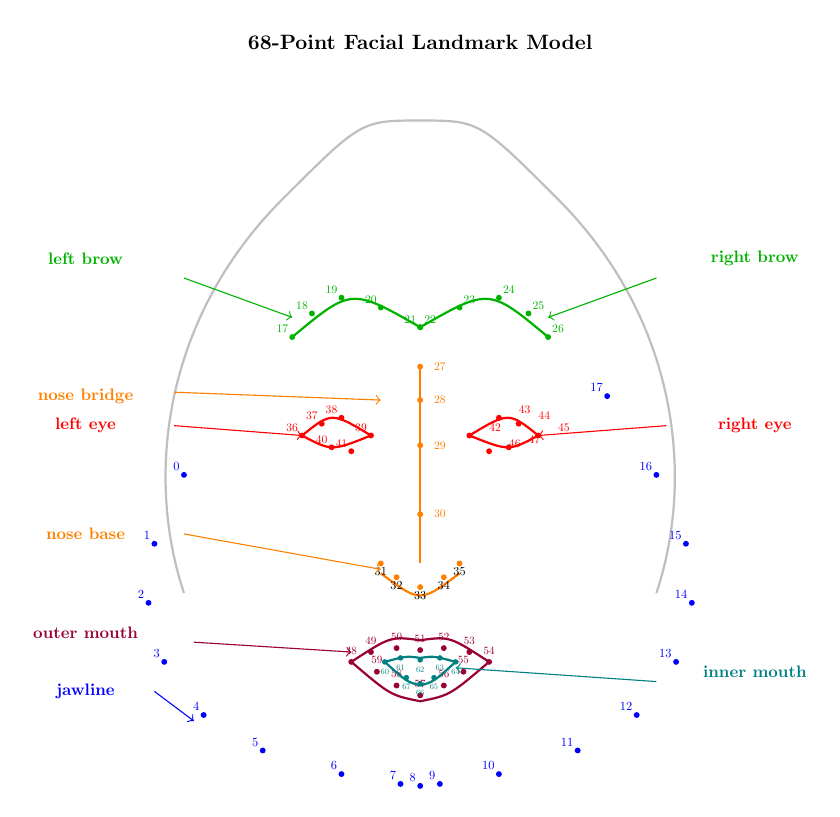
\begin{tikzpicture}[scale=2.5]
        % Face outline (jaw + forehead suggestion)
        \draw[color=gray!50, thick]
            (-1.2, -0.2) .. controls (-1.4, 0.4) and (-1.3, 1.2) .. (-0.7, 1.8)
            .. controls (-0.3, 2.2) .. (0, 2.2)
            .. controls (0.3, 2.2) .. (0.7, 1.8)
            .. controls (1.3, 1.2) and (1.4, 0.4) .. (1.2, -0.2);

        % Jawline points (0-17) — along the lower contour
        \foreach \i/\x/\y in {
            0/-1.2/0.4, 1/-1.35/0.05, 2/-1.38/-0.25, 3/-1.3/-0.55,
            4/-1.1/-0.82, 5/-0.8/-1.0, 6/-0.4/-1.12, 7/-0.1/-1.17,
            8/0/-1.18, 9/0.1/-1.17, 10/0.4/-1.12, 11/0.8/-1.0,
            12/1.1/-0.82, 13/1.3/-0.55, 14/1.38/-0.25, 15/1.35/0.05,
            16/1.2/0.4, 17/0.95/0.8
        }{
            \fill[blue] (\x,\y) circle (0.015);
            \node[scale=0.45, blue, anchor=south east] at (\x,\y) {\i};
        }

        % Left eyebrow (17-21)
        \draw[color=green!70!black, thick] (-0.65, 1.1) .. controls (-0.35, 1.35) .. (0.0, 1.15);
        \foreach \i/\x/\y in {
            17/-0.65/1.1, 18/-0.55/1.22, 19/-0.4/1.3, 20/-0.2/1.25, 21/0.0/1.15
        }{
            \fill[green!70!black] (\x,\y) circle (0.015);
            \node[scale=0.42, green!70!black, anchor=south east] at (\x,\y) {\i};
        }

        % Right eyebrow (22-26)
        \draw[color=green!70!black, thick] (0.0, 1.15) .. controls (0.35, 1.35) .. (0.65, 1.1);
        \foreach \i/\x/\y in {
            22/0.0/1.15, 23/0.2/1.25, 24/0.4/1.3, 25/0.55/1.22, 26/0.65/1.1
        }{
            \fill[green!70!black] (\x,\y) circle (0.015);
            \node[scale=0.42, green!70!black, anchor=south west] at (\x,\y) {\i};
        }

        % Nose bridge (27-30)
        \draw[color=orange, thick] (0, 0.95) -- (0, 0.55) -- (0, 0.2) -- (0, -0.05);
        \foreach \i/\x/\y in {
            27/0/0.95, 28/0/0.78, 29/0/0.55, 30/0/0.2
        }{
            \fill[orange] (\x,\y) circle (0.015);
            \node[scale=0.42, orange, anchor=west] at (\x+0.05,\y) {\i};
        }

        % Nose base (31-35)
        \draw[color=orange, thick] (-0.2,-0.1) .. controls (0,-0.25) .. (0.2,-0.1);
        \foreach \i/\x/\y in {
            31/-0.2/-0.05, 32/-0.12/-0.12, 33/0/-0.17, 34/0.12/-0.12, 35/0.2/-0.05
        }{
            \fill[orange] (\x,\y) circle (0.015);
            \node[scale=0.44, anchor=north] at (\x,\y) {\i};
        }

        % Left eye (36-41)
        \draw[color=red, thick]
            (-0.6, 0.6) .. controls (-0.45, 0.72) .. (-0.25, 0.6)
            .. controls (-0.45, 0.52) .. (-0.6, 0.6);
        \foreach \i/\x/\y in {
            36/-0.6/0.6, 37/-0.5/0.66, 38/-0.4/0.69, 39/-0.25/0.6,
            40/-0.45/0.54, 41/-0.35/0.52
        }{
            \fill[red] (\x,\y) circle (0.015);
            \node[scale=0.42, red, anchor=south east] at (\x,\y) {\i};
        }

        % Right eye (42-47)
        \draw[color=red, thick]
            (0.25, 0.6) .. controls (0.45, 0.72) .. (0.6, 0.6)
            .. controls (0.45, 0.52) .. (0.25, 0.6);
        \foreach \i/\x/\y in {
            42/0.25/0.6, 43/0.4/0.69, 44/0.5/0.66, 45/0.6/0.6,
            46/0.35/0.52, 47/0.45/0.54
        }{
            \fill[red] (\x,\y) circle (0.015);
            \node[scale=0.42, red, anchor=south west] at (\x+0.08,\y) {\i};
        }

        % Outer mouth (48-59)
        \draw[color=purple!80!black, thick]
            (-0.35, -0.55) .. controls (-0.15, -0.42) .. (0, -0.44)
            .. controls (0.15, -0.42) .. (0.35, -0.55)
            .. controls (0.15, -0.72) .. (0, -0.75)
            .. controls (-0.15, -0.72) .. (-0.35, -0.55);
        \foreach \i/\x/\y in {
            48/-0.35/-0.55, 49/-0.25/-0.50, 50/-0.12/-0.48, 51/0/-0.49,
            52/0.12/-0.48, 53/0.25/-0.50, 54/0.35/-0.55,
            55/0.22/-0.60, 56/0.12/-0.67, 57/0/-0.72,
            58/-0.12/-0.67, 59/-0.22/-0.60
        }{
            \fill[purple!80!black] (\x,\y) circle (0.015);
            \node[scale=0.4, purple!80!black, anchor=south] at (\x,\y+0.02) {\i};
        }

        % Inner mouth (60-67)
        \draw[color=teal, thick]
            (-0.18, -0.55) .. controls (-0.07, -0.52) .. (0, -0.53)
            .. controls (0.07, -0.52) .. (0.18, -0.55)
            .. controls (0.07, -0.65) .. (0, -0.67)
            .. controls (-0.07, -0.65) .. (-0.18, -0.55);
        \foreach \i/\x/\y in {
            60/-0.18/-0.55, 61/-0.10/-0.53, 62/0/-0.54, 63/0.10/-0.53,
            64/0.18/-0.55, 65/0.07/-0.63, 66/0/-0.66, 67/-0.07/-0.63
        }{
            \fill[teal] (\x,\y) circle (0.014);
            \node[scale=0.3, teal, anchor=north] at (\x,\y-0.02) {\i};
        }

        % Region labels with arrows
        \node[blue, scale=0.6, font=\bfseries] at (-1.7, -0.7) {jawline};
        \draw[blue, ->, thin] (-1.35, -0.7) -- (-1.15, -0.85);

        \node[green!70!black, scale=0.6, font=\bfseries] at (-1.7, 1.5) {left brow};
        \draw[green!70!black, ->, thin] (-1.2, 1.4) -- (-0.65, 1.2);

        \node[green!70!black, scale=0.6, font=\bfseries] at (1.7, 1.5) {right brow};
        \draw[green!70!black, ->, thin] (1.2, 1.4) -- (0.65, 1.2);

        \node[orange, scale=0.6, font=\bfseries] at (-1.7, 0.8) {nose bridge};
        \draw[orange, ->, thin] (-1.25, 0.82) -- (-0.2, 0.78);

        \node[orange, scale=0.6, font=\bfseries] at (-1.7, 0.1) {nose base};
        \draw[orange, ->, thin] (-1.2, 0.1) -- (-0.2, -0.08);

        \node[red, scale=0.6, font=\bfseries] at (-1.7, 0.65) {left eye};
        \draw[red, ->, thin] (-1.25, 0.65) -- (-0.6, 0.6);

        \node[red, scale=0.6, font=\bfseries] at (1.7, 0.65) {right eye};
        \draw[red, ->, thin] (1.25, 0.65) -- (0.6, 0.6);

        \node[purple!80!black, scale=0.6, font=\bfseries] at (-1.7, -0.4) {outer mouth};
        \draw[purple!80!black, ->, thin] (-1.15, -0.45) -- (-0.35, -0.50);

        \node[teal, scale=0.6, font=\bfseries] at (1.7, -0.6) {inner mouth};
        \draw[teal, ->, thin] (1.2, -0.65) -- (0.18, -0.58);

        % Title
        \node[font=\bfseries, scale=0.75] at (0, 2.6) {68-Point Facial Landmark Model};
    \end{tikzpicture}
    \caption{Schematic diagram of the 68-point facial landmark model. Each colour corresponds to a different facial region. Points are numbered according to the iBUG 300-W convention.}
    \label{fig:landmark-68}
\end{figure}

\subsection{How Landmark Detectors Work}

Landmark detection algorithms take an image (or a cropped face region) as input and output a set of 2D coordinates $\{(x_i, y_i)\}_{i=0}^{67}$ for the 68-point model. Three approaches are particularly noteworthy.

\subsubsection*{HOG + SVM + Regressed Trees (dlib Classic)}

This pipeline, popularized by the widely used \texttt{dlib} library~\footnote{See the dlib library documentation for details on the HOG+SVM face detector.}, works in two stages:

\begin{enumerate}
    \item \textbf{Face detection with HOG + linear SVM.} A \textbf{Histogram of Oriented Gradients} feature descriptor is computed on sliding windows across the image. Each window's HOG feature vector is classified by a \textbf{Support Vector Machine} trained to distinguish face regions from background. The result is a bounding box around the detected face.
    \item \textbf{Landmark localization with cascaded regression.} Given the bounding box, a cascade of \textbf{regression trees} iteratively refines the landmark positions. Starting from an initial estimate (often the mean shape from the training data), each tree in the cascade predicts a correction $\Delta$ to the current landmark positions:
    \begin{equation}
        \mathbf{s}_{t+1} = \mathbf{s}_t + \Delta_t(\mathbf{I}, \mathbf{s}_t),
    \end{equation}
    where $\mathbf{s}_t$ is the shape at iteration $t$, $\mathbf{I}$ is the image, and $\Delta_t$ is the $t$-th regressor's prediction. After typically 5--10 iterations, the landmarks converge to stable positions.
\end{enumerate}

\textbf{Pros:} Very fast (runs in real time on a CPU), small model size. \\
\textbf{Cons:} Less accurate than deep learning methods, especially for non-frontal faces or unusual expressions.

\subsubsection*{Deep Neural Network (dlib CNN)}

The same \texttt{dlib} library also provides a CNN-based landmark detector~\footnote{One Millisecond Face Alignment with an Ensemble of Regression Trees, Kazemi \& Sullivan, CVPR 2014.}. This model replaces the hand-crafted HOG features and decision-tree cascade with a single \textbf{end-to-end convolutional neural network} that takes a normalized face patch as input and directly outputs the 68 landmark coordinates (136 real values).

Because the network learns features from data rather than relying on histogram statistics, it is significantly more robust to variations in lighting, pose, and expression.

\textbf{Pros:} Higher accuracy, better handling of partial occlusions and extreme poses. \\
\textbf{Cons:} Slower than the HOG-based approach (though still CPU-feasible), larger model footprint.

\subsubsection*{MediaPipe Face Mesh (Google)}

Google's MediaPipe framework~\footnote{MediaPipe is Google's open-source framework for multimodal ML models, including real-time face mesh detection.} takes a different approach: instead of 68 points, it predicts \textbf{477 3D facial landmarks}, providing much denser coverage across the entire face surface. It uses a multi-stage pipeline:

\begin{enumerate}
    \item \textbf{BlazeFace detector:} A lightweight neural network quickly locates the face and produces a rough bounding box (with sub-millisecond latency).
    \item \textbf{Face Mesh model:} A deeper CNN takes the cropped face region and predicts the full 477-point mesh, including 3D coordinates $(x, y, z)$ where $z$ represents depth relative to the image plane.
\end{enumerate}

The 477 points cover the entire facial surface: contours, eyes, eyebrows, nose, lips, teeth, and even sub-regions of the iris. This density is useful for high-fidelity morphing and augmented reality, though it introduces additional computational complexity.

\textbf{Pros:} Extremely dense coverage, 3D depth information, real-time on mobile devices, robust across diverse lighting and pose conditions. \\
\textbf{Cons:} Overkill for basic morphing (most morphing workflows only need $\sim$68 points), output must be subsampled or mapped to the 68-point convention for compatibility.

\subsection{Coordinate System}

All landmark coordinates are expressed in the standard \textbf{image coordinate system}. Unlike the Cartesian coordinate system taught in mathematics class, image coordinates have the following convention:

\begin{itemize}
    \item The \textbf{origin} $(0, 0)$ is at the \textbf{top-left corner} of the image.
    \item The $x$-axis increases \textbf{rightward}.
    \item The $y$-axis increases \textbf{downward}.
\end{itemize}

Landmark coordinates are stored as \textbf{floating-point values in pixel units}. This means that a landmark at $(x, y) = (150.5, 200.3)$ refers to a sub-pixel location 150.5~pixels from the left edge and 200.3~pixels from the top edge. Sub-pixel precision is important because warping operations work with fractional coordinates.

Figure~\ref{fig:coord-system} illustrates this coordinate system.

\begin{figure}[htbp]
    \centering
    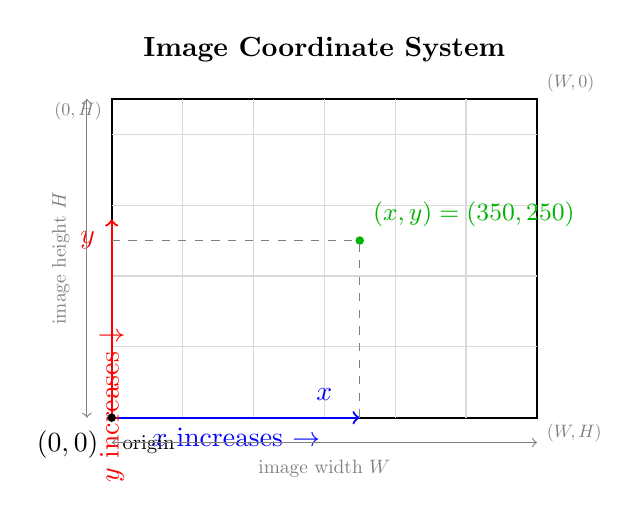
\begin{tikzpicture}[scale=0.9]
        % Image rectangle
        \draw[thick] (0,0) rectangle (6,4.5);

        % Grid lines (subtle)
        \foreach \x in {1,...,5} {
            \draw[gray!30] (\x,0) -- (\x,4.5);
        }
        \foreach \y in {1,...,4} {
            \draw[gray!30] (0,\y) -- (6,\y);
        }

        % Axes
        \draw[->, thick, blue] (0,0) -- (3.5,0) node[midway, below, sloped] {$x$ increases \(\rightarrow\)};
        \draw[->, thick, red] (0,0) -- (0,2.8) node[midway, left, sloped] {$y$ increases \(\downarrow\)};

        % Origin
        \fill[black] (0,0) circle (0.06);
        \node[anchor=north east, font=\bfseries] at (-0.05, -0.05) {$(0,0)$};
        \node[anchor=north west, scale=0.75] at (0.05, -0.15) {origin};

        % Axis labels
        \node[anchor=south, blue, font=\bfseries] at (3,0.1) {$x$};
        \node[anchor=east, red, font=\bfseries] at (-0.1,2.5) {$y$};

        % Example landmark point
        \fill[green!70!black] (3.5,2.5) circle (0.06);
        \node[anchor=south west, green!70!black, font=\small] at (3.55, 2.55) {\small$(x, y) = (350, 250)$};
        \draw[dashed, gray] (3.5,0) -- (3.5,2.5);
        \draw[dashed, gray] (0,2.5) -- (3.5,2.5);

        % Pixel dimensions annotation
        \node[anchor=north, gray, scale=0.7] at (3, -0.5) {image width $W$};
        \draw[gray, <->] (0, -0.35) -- (6, -0.35);
        \node[anchor=east, gray, scale=0.7] at (-0.5, 2.25) {\rotatebox{90}{image height $H$}};
        \draw[gray, <->] (-0.35, 0) -- (-0.35, 4.5);

        % Top-right corner
        \node[anchor=south west, gray, scale=0.65] at (6.05, 4.5) {$(W, 0)$};
        \node[anchor=north west, gray, scale=0.65] at (6.05, 0) {$(W, H)$};
        \node[anchor=north east, gray, scale=0.65] at (-0.05, 4.55) {$(0, H)$};

        % Title
        \node[font=\bfseries] at (3, 5.2) {Image Coordinate System};
    \end{tikzpicture}
    \caption{The image coordinate system used for landmarks. The origin is at the top-left corner, $x$ increases rightward, and $y$ increases downward. An example landmark at $(350, 250)$ is shown in green.}
    \label{fig:coord-system}
\end{figure}

\begin{remark}
    When working with multiple detector libraries, be aware of coordinate conventions. Some libraries return landmarks in \emph{normalized} coordinates $[0, 1]$ relative to the face bounding box, rather than absolute pixel coordinates. Always check the API documentation and convert coordinates to your preferred frame before warping.
\end{remark}

\subsection{Preprocessing for Better Detection}

Landmark detectors are sensitive to the quality of the input face image. Although modern detectors are fairly robust, following a few simple preprocessing guidelines will significantly improve detection accuracy \emph{and} downstream morphing quality.

\paragraph*{Why good face detection and cropping matters.}

All landmark models are trained on face images that share certain properties:
\begin{itemize}
    \item \textbf{The face is roughly front-facing.} Extreme side profiles (more than $\sim45^\circ$ rotation) cause many landmarks to be occluded and therefore poorly localized.
    \item \textbf{The face is large enough in the frame.} As a rule of thumb, the cropped face should be at least $200 \times 200$ pixels. Below this, pixel-level detail around the eyes, lips, and nose is insufficient for precise localization.
    \item \textbf{The face is roughly centred and upright.} Large in-plane rotations (tilting your head sideways) confuse detectors because the statistical priors assume an upright face.
\end{itemize}

A typical preprocessing pipeline for morphing therefore looks like this:
\begin{enumerate}
    \item \textbf{Detect} the face bounding box (using any face detector).
    \item \textbf{Crop} a square region around the face with some margin (e.g., 20\% padding on each side).
    \item \textbf{Align} by rotating the image so that the eyes are horizontally level. This can be done by computing the angle $\theta = \arctan\!\big((y_R - y_L)/(x_R - x_L)\big)$ between the two eye centres and applying a rotation.
    \item \textbf{Resize} to a standard resolution (e.g., $512 \times 512$ pixels) so that landmark coordinates are comparable across images.
    \item \textbf{Run the landmark detector} on the preprocessed face.
\end{enumerate}

The result is a set of landmarks that are accurate, consistent, and ready for computing the correspondence needed to morph two faces together---the subject of the next section.
